% the template is adapted from https://github.com/kourgeorge/arxiv-style

\documentclass{article}


\usepackage{arxiv}

\usepackage[utf8]{inputenc} % allow utf-8 input
\usepackage[T1]{fontenc}    % use 8-bit T1 fonts
\usepackage{hyperref}       % hyperlinks
\usepackage{url}            % simple URL typesetting
\usepackage{booktabs}       % professional-quality tables
\usepackage{amsfonts}       % blackboard math symbols
\usepackage{nicefrac}       % compact symbols for 1/2, etc.
\usepackage{microtype}      % microtypography
\usepackage{lipsum}		% Can be removed after putting your text content

\usepackage{tikz} 
\usetikzlibrary{matrix}

\usepackage{graphicx}
%\usepackage{hyperref}
\usepackage{amsmath,amssymb}
\usepackage{algorithm}
%\usepackage{algorithmicx}
%\usepackage{algpseudocode}
\usepackage{subcaption}
%\usepackage{booktabs}


\title{Some not that novel approach to image processing using nonparametric statistic}


%\date{September 9, 1985}	% Here you can change the date presented in the paper title
%\date{} 					% Or removing it

\author{
  Zhuo Yueyi \\ %\thanks{Use footnote for providing further
    %information about author (webpage, alternative
    %address)---\emph{not} for acknowledging funding agencies.} \\
  Department of Computer Science and Engineering\\
  Nanjing University of Science and Technology\\
  \texttt{yiyuezhuo@gmail.com} \\
}

\begin{document}
\maketitle

\begin{abstract}
%\lipsum[1]
This is a class paper for nonparametric statistical. 
All of methods introduced by \cite{wasserman2006all} will get a example to show how it can be applied on
image processing problem.
\end{abstract}


% keywords can be removed
\keywords{Nonparametric statistic \and image processing }


\section{Introduction}
%\lipsum[2]
%\lipsum[3]




\subsection{Data format of image}
%\label{sec:headings}
%\lipsum[4] See Section \ref{sec:headings}.

Colored(RGB) image can seen as a 3 variables function  $f(i,j,c)$, where $i,j$ denote the location of image, $c$ denotes
channel(reg, green, blue). The function can be encoded by three matrixes as shown in Fig~\ref{fig:toad_rgb}.

\begin{figure}[htb]
  \centering
  \begin{tikzpicture}
    \node[inner sep=0pt] (toad_rgb) at (-2.5,0)
    {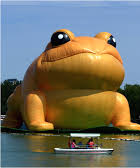
\includegraphics[width=.15\textwidth]{images/toad_rgb.png}};
    \node[inner sep=0pt] (toad_r) at (0.0,0)
    {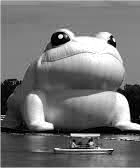
\includegraphics[width=.15\textwidth]{images/toad_r.png}};
    \node[inner sep=0pt] (toad_g) at (2.5,0)
    {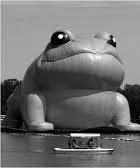
\includegraphics[width=.15\textwidth]{images/toad_g.png}};
    \node[inner sep=0pt] (toad_b) at (5.0,0)
    {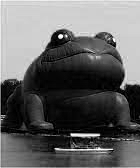
\includegraphics[width=.15\textwidth]{images/toad_b.png}};
    
    \draw [->] (toad_rgb.south) to [out=355, in=185] (toad_r.south);
    \draw [->] (toad_rgb.south) to [out=350, in=190] (toad_g.south);
    \draw [->] (toad_rgb.south) to [out=345, in=195] (toad_b.south);

    % small crop in toad_b
    %\draw [red] (7.5, 0.05) -- (7.6, 0.05) -- (7.6,-0.05) -- (7.5, -0.05) -- (7.5, 0.05);
    \draw [red] ([shift={(0.0, 0.05)}]toad_b.center) --
      ([shift={(0.1, 0.05)}]toad_b.center) --
      ([shift={(0.1, -0.05)}]toad_b.center) --
      ([shift={(0.0, -0.05)}]toad_b.center) --
      ([shift={(0.0, 0.05)}]toad_b.center);

    %\node (10.0,0.0) {$$\begin{bmatrix} 1 & 1 \\ 2 & 2 \end{bmatrix}$$};
    \matrix [matrix of nodes,row sep=-1ex, column sep=-1ex] (toad_mat) at (7.7, 0.0)
    {
        5 & 7 & 10 & 10 & 11 & 4 \\
        6 & 8 & 8 & 10 & 10 & 5 \\
        5 & 6 & 8 & 8 & 7 & 4 \\
        6 & 5 & 6 & 5 & 7 & 5 \\
        6 & 6 & 4 & 5 & 4 & 4 \\
        5 & 5 & 4 & 2 & 3 & 6  \\  };

    \draw [->] ([shift={(0.1, 0.05)}]toad_b.center) -- (toad_mat.north west);
    \draw [->] ([shift={(0.1, -0.05)}]toad_b.center) -- (toad_mat.south west);

    % draw matrix frame, how stupid I need to write it manually.
    \draw ([shift={(0.15, 0.0)}]toad_mat.north west) -- 
        ([shift={(0.05, 0.0)}]toad_mat.north west) --
        ([shift={(0.05, 0.0)}]toad_mat.south west) --
        ([shift={(0.15, 0.0)}]toad_mat.south west);

    \draw ([shift={(-0.15, 0.0)}]toad_mat.north east) -- 
        ([shift={(-0.05, 0.0)}]toad_mat.north east) --
        ([shift={(-0.05, 0.0)}]toad_mat.south east) --
        ([shift={(-0.15, 0.0)}]toad_mat.south east);

    \node at ([shift={(0.0, 0.2)}]toad_rgb.north) {RGB};
    \node at ([shift={(0.0, 0.2)}]toad_r.north) {R};
    \node at ([shift={(0.0, 0.2)}]toad_g.north) {G};
    \node at ([shift={(0.0, 0.2)}]toad_b.north) {B};
    \node at ([shift={(0.0, 0.2)}]toad_mat.north) {matrix of the crop};
    
    % two example equation to show the function sematic
    \node (eq1) at  (10.0, 0.2) {$f(84, 72, 2)$};
    \node (eq2) at  (10.0,-0.2) {$f(85, 72, 2)$};

    \draw [->] ([shift={(-0.2, 0.2)}]toad_mat.east) -- (eq1);
    \draw [->] ([shift={(-0.2, -0.2)}]toad_mat.east) -- (eq2);

    %\draw[help lines] (0,0) grid (10,-10);
\end{tikzpicture}

  \caption{Representation: Image as three matrix}
  \label{fig:toad_rgb}
\end{figure}

Since the colored image introduce extra complexity, in this paper the gray image is used for simplicity.
Instead of three matrices, the gray image is represented by a single matrix which is given by:

$$
f_{gray}(i,j) = 0.21 f_{rgb}(i,j,1) + 0.72 f_{rgb}(i,j,2) + 0.07 f_{rgb}(i,j,3)
$$

Sometimes to "flatten" a matrix to a long vector is a useful viewpoint. There're two order to flatten a matrix,
row-major and column-major. The row-major is used in Python(Numpy) and the column-major is used by R and MatLab.
As my preferred language, row-major order of Python is illustrated as Fig~\ref{fig:flatten_matrix}.

\begin{figure}[htb]
  \centering
  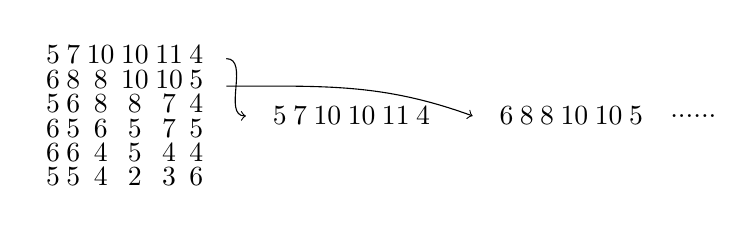
\begin{tikzpicture}
    \matrix [matrix of nodes,row sep=-1ex, column sep=-1ex, anchor=west] (toad_mat) at (0.0, 0.0)
    {
        5 & 7 & 10 & 10 & 11 & 4 \\
        6 & 8 & 8 & 10 & 10 & 5 \\
        5 & 6 & 8 & 8 & 7 & 4 \\
        6 & 5 & 6 & 5 & 7 & 5 \\
        6 & 6 & 4 & 5 & 4 & 4 \\
        5 & 5 & 4 & 2 & 3 & 6  \\  };
    
    \matrix [matrix of nodes,row sep=-1ex, column sep=-1ex, anchor=west] (toad_r1) at ([shift={(0.4, 0.00)}]toad_mat.east)
    {
        5 & 7 & 10 & 10 & 11 & 4 \\};

    \matrix [matrix of nodes,row sep=-1ex, column sep=-1ex, anchor=west] (toad_r2) at ([shift={(0.4, 0.00)}]toad_r1.east)
    {
        6 & 8 & 8 & 10 & 10 & 5 \\};
    
    \node (ellipsis) at  ([shift={(0.4, 0.00)}]toad_r2.east) {......};

    %\draw [->] ([shift={(0.05, 0.00)}]toad_mat.east ) -- ([shift={(-0.1, 0.00)}]toad_r1.west);
    %\draw [->] ([shift={(0.05, -0.60)}]toad_mat.east ) -- ([shift={(-0.1, 0.00)}]toad_r2.west);
    \draw [->] ([shift={(0.05, -0.40)}]toad_mat.north east) to [out=0, in=180] ([shift={(-0.1, 0.00)}]toad_r1.west);
    \draw [->] ([shift={(0.05, -0.75)}]toad_mat.north east) to [out=0, in=160] ([shift={(-0.1, 0.00)}]toad_r2.west);

\end{tikzpicture}

  \caption{Flatten a matrix by row}
  \label{fig:flatten_matrix}
\end{figure}


As a application we can model the vector as i.i.d sample of some distribution using simpler symbol, the most 
common practice is to represent them as a histogram, see Fig~\ref{fig:map_gray_to_hist}.

\begin{figure}[htb]
  \centering
  \begin{tikzpicture}
    \node[inner sep=0pt, anchor=west] (toad_gray) at (0,0)
    {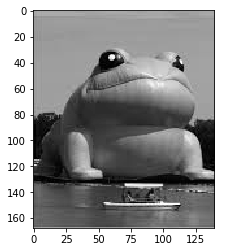
\includegraphics[width=.15\textwidth]{images/toad_gray.png}};
    \node[inner sep=0pt, anchor=west] (toad_hist) at ([shift={(0.5, 0.0)}]toad_gray.east)
    {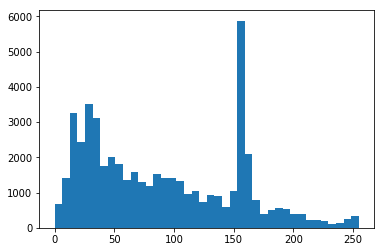
\includegraphics[width=.15\textwidth]{images/toad_hist.png}};

    \draw [->] (toad_gray.east) -- (toad_hist.west);

\end{tikzpicture}

  \caption{Mapping from gray image to histogram}
  \label{fig:map_gray_to_hist}
\end{figure}

\subsection{Inverse problem in image processing}

As presented in \cite{dong2015image}, we usually regard image as a result of combination of some "observe"
function and noise. In its simplest form, we can write:

\begin{equation}
\mathbf{f} = \mathbf{A} \mathbf{x} + \mathbf{\eta}
\label{eq:inverse_problem}
\end{equation}

where $\mathbf{f}$ denote a (gray) image, $\mathbf{A}$ is a linear operation, $\mathbf{x}$ is "true" image,
$\mathbf{\eta}$ is noise.
 
\section{Smoothing: nonparametric statistic and image processing}

There exists a fully equivalence which can be shown on smoothing problem.

\cite{wasserman2006all} state regression for pairs $(x_1,Y_1,\dots,x_n,Y_n)$ like:

$$
Y_i = r(x_i) + \epsilon_i
$$

Replacing $x_i$ with $x_{ij}=(i,j)$ ($i,j$ denote coordinates of corresponding pixel on image), compared to Eq~\ref{eq:inverse_problem},
so the $r(x_{i,j})=r(i,j)$ denote the complex true image function. 
It's obvious that we can not specify a simple parametric model on it (For some possible parametric image model,
see Fig~\ref{fig:parametric_model} ) so that the the noise derived from underestimated model will cause misunderstanding. 
Thus we must employ a nonparametric fashion though computer scientist may not aware it explicitly.

\begin{figure}[htb]
  \centering
  \begin{subfigure}[b]{0.24\linewidth}
    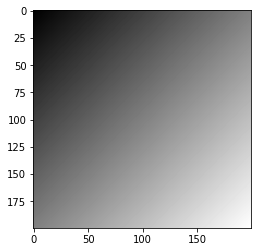
\includegraphics[width=\linewidth]{images/parametric_model_1.png}
    \caption{$y_{ij} = i+j$}
  \end{subfigure}
  \begin{subfigure}[b]{0.24\linewidth}
    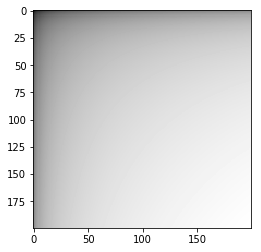
\includegraphics[width=\linewidth]{images/parametric_model_2.png}
    \caption{$y_{ij} = \log(1+i)+\log(1+j)$}
  \end{subfigure}
  \begin{subfigure}[b]{0.24\linewidth}
    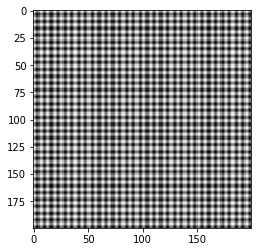
\includegraphics[width=\linewidth]{images/parametric_model_3.png}
    \caption{$y_{ij} = \sin(i)+\sin(j)$}
  \end{subfigure}
  \begin{subfigure}[b]{0.24\linewidth}
    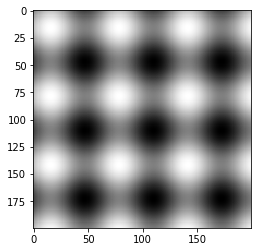
\includegraphics[width=\linewidth]{images/parametric_model_4.png}
    \caption{$y_{ij} = \sin(0.1i)+\sin(0.1j)$}
  \end{subfigure}
  \caption{Simple parametric model can't capture big picture of image.}
  \label{fig:parametric_model}
\end{figure}


\subsection{Kernel regression}
%\lipsum[5]
%\begin{equation}
%\xi _{ij}(t)=P(x_{t}=i,x_{t+1}=j|y,v,w;\theta)= {\frac {\alpha _{i}(t)a^{w_t}_{ij}\beta _{j}(t+1)b^{v_{t+1}}_{j}(y_{t+1})}{\sum _{i=1}^{N} \sum _{j=1}^{N} \alpha _{i}(t)a^{w_t}_{ij}\beta _{j}(t+1)b^{v_{t+1}}_{j}(y_{t+1})}}
%\end{equation}

As stated in \cite{solomon2011fundamentals}, a mean filtering, as simplest filter technology, give same weight to neibor pixel to smooth the
noised to remove noise(try to find true$r(i,j)$). Concretely, here's a instance of $3 \times 3$ filtering:

\begin{equation}
g(i,j) = \frac{1}{9} \sum_{di=-1}^1 \sum_{dj=-1}^1 f(i+di,j+dj)
\label{eq:mean_filter}
\end{equation}

If we set kernel function as:

$$ 
K(x_{i,j},y_{i,j}) =  
\begin{cases}
  1, & \text{if $ |i_x - i_y| \le 1$ and $|j_x - j_y| \le 1$} \\
  0, & \text{otherwise}
\end{cases}
$$

Which is a nature two-variables extension from box-car kernel introduced by \cite{wasserman2006all}.
Then the kernel regression given by:

$$
\hat{r}(x_{i,j}) = \frac{\sum_{s} \sum_{t} K(x_{i,j},x_{s,t}) Y_{s,t}}{\sum_{s} \sum_{t} K(x_{i,j},x_{s,t})}
$$

is equivalence to Eq~\ref{eq:mean_filter}. A example can be shown in Fig~\ref{fig:effect_noise_removal}. 
The kernel size(here it's $3$) is directly correspond to bandwidth $h$ used in kernel regression.

Mean filtering is usually weaker than median filtering, a example is shown in Fig~\ref{fig:effect_noise_removal}. 
Though median filtering is also a linear smoother $\hat{r}(x_{i,j})=\sum_s \sum_t l_{s,t}(x_{i,j})Y_{s,t}$, 
a instance of its hat-matrix may be $ l_{s,t}(x_{i,j}) = I(s=i_{median}) \times I(t=j_{median}) $. 
Where $i_{median},j_{median}$ denote the coordinates of pixel which is median of neiborhood of given pixel $(i,j)$.

But obviously it can not be included by kernel regression, say, 
we can't find a general kernel function $K(x_{i,j},y_{i,j})$ which give above hat matrix. 

Following textbook \cite{wasserman2006all}, we can try to find different improvment other than mean-filter 
or rank-filter, for example, local regression. 

\begin{figure}[htb]
  \centering
  \begin{subfigure}[b]{0.24\linewidth}
    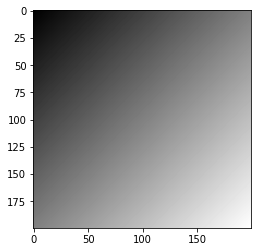
\includegraphics[width=\linewidth]{images/parametric_model_1.png}
    \caption{Kernel regression(h=1)}
  \end{subfigure}
  \begin{subfigure}[b]{0.24\linewidth}
    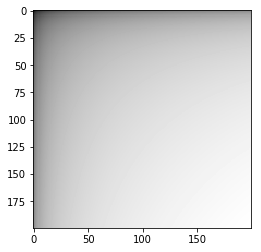
\includegraphics[width=\linewidth]{images/parametric_model_2.png}
    \caption{Kernel regression(h=10)}
  \end{subfigure}
  \begin{subfigure}[b]{0.24\linewidth}
    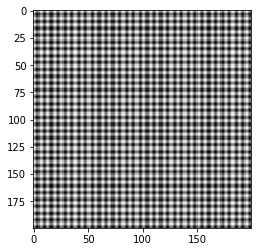
\includegraphics[width=\linewidth]{images/parametric_model_3.png}
    \caption{Median regression}
  \end{subfigure}
  \begin{subfigure}[b]{0.24\linewidth}
    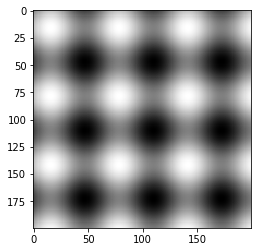
\includegraphics[width=\linewidth]{images/parametric_model_4.png}
    \caption{Local regression}
  \end{subfigure}
  \caption{Simple parametric model can't capture big picture of image.}
  \label{fig:effect_noise_removal}
\end{figure}


\subsection{Local Regression}

\subsection{Variance estimation introduced by smoothing}

\subsubsection{Headings: third level}
\lipsum[6]

\paragraph{Paragraph}
\lipsum[7]

\section{Examples of citations, figures, tables, references}
\label{sec:others}
\lipsum[8] \cite{kour2014real,kour2014fast} and see \cite{hadash2018estimate}.

The documentation for \verb+natbib+ may be found at
\begin{center}
  \url{http://mirrors.ctan.org/macros/latex/contrib/natbib/natnotes.pdf}
\end{center}
Of note is the command \verb+\citet+, which produces citations
appropriate for use in inline text.  For example,
\begin{verbatim}
   \citet{hasselmo} investigated\dots
\end{verbatim}
produces
\begin{quote}
  Hasselmo, et al.\ (1995) investigated\dots
\end{quote}

\begin{center}
  \url{https://www.ctan.org/pkg/booktabs}
\end{center}


\subsection{Figures}
\lipsum[10] 
See Figure \ref{fig:fig1}. Here is how you add footnotes. \footnote{Sample of the first footnote.}
\lipsum[11] 



\subsection{Tables}
\lipsum[12]
See awesome Table~\ref{tab:table}.

\begin{table}
 \caption{Sample table title}
  \centering
  \begin{tabular}{lll}
    \toprule
    \multicolumn{2}{c}{Part}                   \\
    \cmidrule(r){1-2}
    Name     & Description     & Size ($\mu$m) \\
    \midrule
    Dendrite & Input terminal  & $\sim$100     \\
    Axon     & Output terminal & $\sim$10      \\
    Soma     & Cell body       & up to $10^6$  \\
    \bottomrule
  \end{tabular}
  \label{tab:table}
\end{table}

\subsection{Lists}
\begin{itemize}
\item Item 1 Item 2
\item Item 3 Item 4
\item Item 5 Item 6
\end{itemize}


\bibliographystyle{unsrt}  
\bibliography{references}  %%% Remove comment to use the external .bib file (using bibtex).
%%% and comment out the ``the bibliography'' section.


\end{document}
